\chapter{NULLと三値論理}

SQLで用いられる値には、NULLというものがあります。では、NULLはどのような意味を持つのでしょうか。また、NULLを判定に使うというのは、どのようなことなのでしょうか。

この章では、少しばかりわかりにくいNULLのはなしをします。

\section{SQLとNULL}

リレーショナルデータベースのテーブルのアトリビュートとして、NULLというものがあります。このNULLは、あるレコードのアトリビュートに入れるべき値が無いときに使われるものです。

テーブルをCREATEするときに、アトリビュートにNOT NULL制約をつけて、NULLを許容しないようにすることができます。また、NULLは、リレーショナルデータベースで許容すべきか否か、という根本的な問題もあります。そんなNULLとは、どんな存在なのでしょうか。

たとえば、二つのアトリビュートをもつテーブルがあり、あるレコードについては、その一つしか値が決まらなかったとします。そのレコードについて、もうひとつの、値が決まっていないアトリビュートに入っている値がNULLです。

その一方で、あるテーブルにおいて、全てのアトリビュートがNULLであるレコードは存在しません。レコードの情報がなにも無い、ということイコール、そんなレコードは存在しない、ということだからです。つまり、アトリビュートにNULLをとるレコードは、少なくともひとつのアトリビュートは、NULLでない値が入っていなければならないということになります。

コンピュータの言語では、変数などの値が設定されていない状態をさして、NULLである、という言い方をします。また、ポインタの値として、NULLで初期化し、積極的に未設定であることをアピールすることもあります。




\subsection{NULLの意味}

では、リレーショナルデータベースとSQLで、NULLはなにをあらわしているのでしょうか。NULLの意味はふたつあります。ひとつは、それについては知らないという情報を表す値であると言うことです。そして、もうひとつの意味は、それについて適用できるものが無い、という情報をあらわします。

では、NULLのふたつの意味は、どのように区別されるのでしょうか。

\subsubsection{知らないというNULL}

\begin{figure}[htbp]
	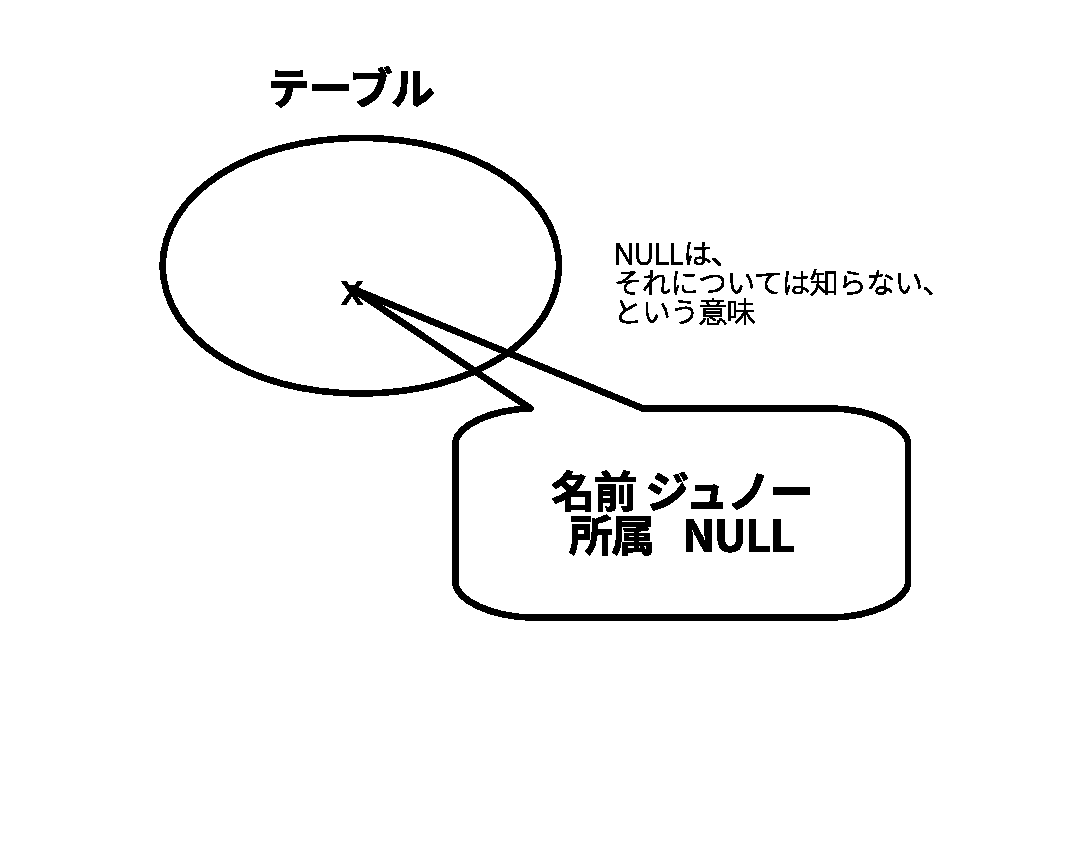
\includegraphics[width=12cm,clip]{draw/null.eps}
	\caption{NULLをもつレコード}
	\label{fig:record_with_null}
\end{figure}
たとえば、名前と所属という二つのアトリビュートをもつテーブルを考えます。あるレコードで、所属の値がNULLであれば、それは、所属が分からない、という意味になります。

また、レコードにINSERTするとき、アトリビュートの値としてNULLが設定されているということは、その値を決定する情報がない、ということです。このような場合、NULLとは、unknownである、知らないということであると解釈するのが自然です。

\subsubsection{適用できないというNULL}

animalsというテーブルは動物の名前と、動物の種別idをアトリビュートとして持っているとします。kindsテーブルは、idと、動物の種別名を持っています。つまり、kindsは動物の種別名マスターです。

この二つのテーブルは、図\ref{fig:animals_kinds_er}のような関係にあるとします。このとき、animalsに、kindsに種別名が入っていない動物の情報を入れたくなったときはどうしたらよいでしょうか。そのような登録を許さないという流儀もありますが、ここでは、そのような登録を許すことを前提に考えてみます。

動物の種別マスタであるkindsに鳥類の登録がないのですが、animalsにはペンギンを登録します。このとき、kindidはマスタ側にて基油できるものが無いため、NULLとします。

このようなケースでは、animalsのレコードで、アトリビュートkindis.animalsに、ますた側に適用できるものがない、という意味でNULLを入れます。

これは、LEFT JOINやRIGHT JOINといった、左右の外部結合で必要になる考え方です。左右の外部結合は、JOINの結果であるテーブルに、適用できるものがなかった、という意味のNULLを許容します。これについては、後の章で、あらためて説明します。

\begin{figure}[htbp]
	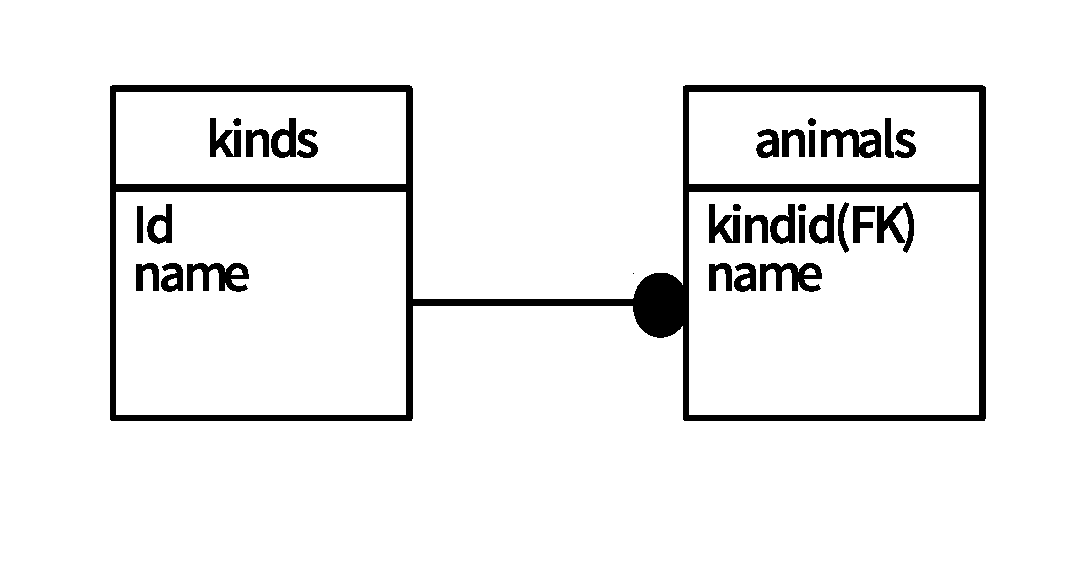
\includegraphics[width=12cm,clip]{draw/null_er.eps}
	\caption{animalsとkindsのER図}
	\label{fig:animals_kinds_er}
\end{figure}

\begin{table}[htb]
  \begin{tabular}{|c|c|} \hline
    id & name \\ \hline
    1 & 哺乳類 \\
    2 & 爬虫類 \\
    3 & 魚類 \\ \hline
  \end{tabular}
  \label{table:kinds}
  \caption{kindsテーブルの内容}
\end{table}

\begin{table}[htb]
  \begin{tabular}{|c|c|} \hline
    kindid & name \\ \hline
    1 & パンダ \\
    2 & 亀 \\
    3 & はまち \\
    NULL & ペンギン \\ \hline
  \end{tabular}
  \label{table:animals}
  \caption{animalsテーブルの内容}
\end{table}


\subsection{NULLの意味の区別}

NULLを使うときに、知らないという意味のNULLと、適用できない、という意味のNULLは、どのように区別すればよいのでしょうか。これは、レコードのアトリビュートの値としては、どちらも同じNULLという値で表されます。

実は、NULLが、知らないと適用できるものがない、どちらの意味で使われているかを、SQLのコードで区別する方法はありません。この意味の違いは文脈的なものであり、どちらの意味で解釈するかはあくまでも人間の判断です。

この二つの意味を区別して、知らないと適用できないを別の値としてあらわそう、という提案もありましたが、結局のところ、リレーショナルデータベースとSQLに、その思想が導入されることはありませんでした。

もうひとつ、NULLを使うときに、現れるいみがあります。それは、情報を入力し忘れて居る場合のNULLです。NULLを使うとき、知らない、適用できないという意味で積極的に使っているNULLなのか、情報を入れ忘れたことで結果的にNULLとなったのか、それを区別する方法はありませんまた、。この意味で使われているかは、文脈から人間が判断することもできません。

\subsection{座標軸とNULL}

これまでで、アトリビュートとは、テーブルという空間の座標軸である、という説明をしてきました。では、値としてNULLをとるとき、そのレコードはテーブルという空間のどこにあるのでしょうか。ここでは、名前と所属という二つのアトリビュートをもつ、テーブルのレコードを考えます。
また、テーブルの空間は、便宜的に平面の直交座標で表され、それぞれ名前の軸と、所属の軸であるとします。

\begin{figure}[htbp]
	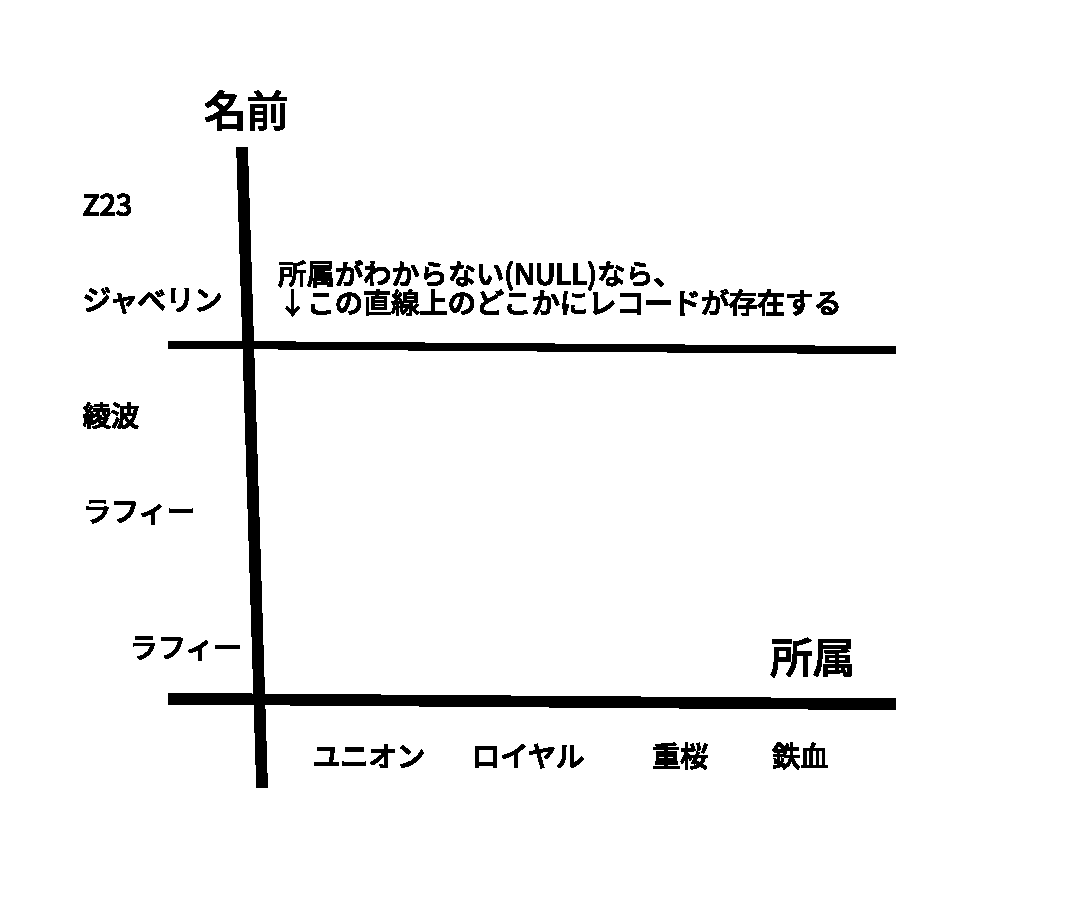
\includegraphics[width=12cm,clip]{draw/unknown.eps}
	\caption{知らないNULLと座標}
	\label{fig:unknown_null}
\end{figure}

知らない、という意味のNULLのときは、ある範囲までしか場所が特定できな、という様に考えることができます。この場合、レコードは、名前の座標軸上の特定の点を通り、所属の座標軸に平行な直線上のどこかにある、というように解釈できます。

\begin{figure}[htbp]
	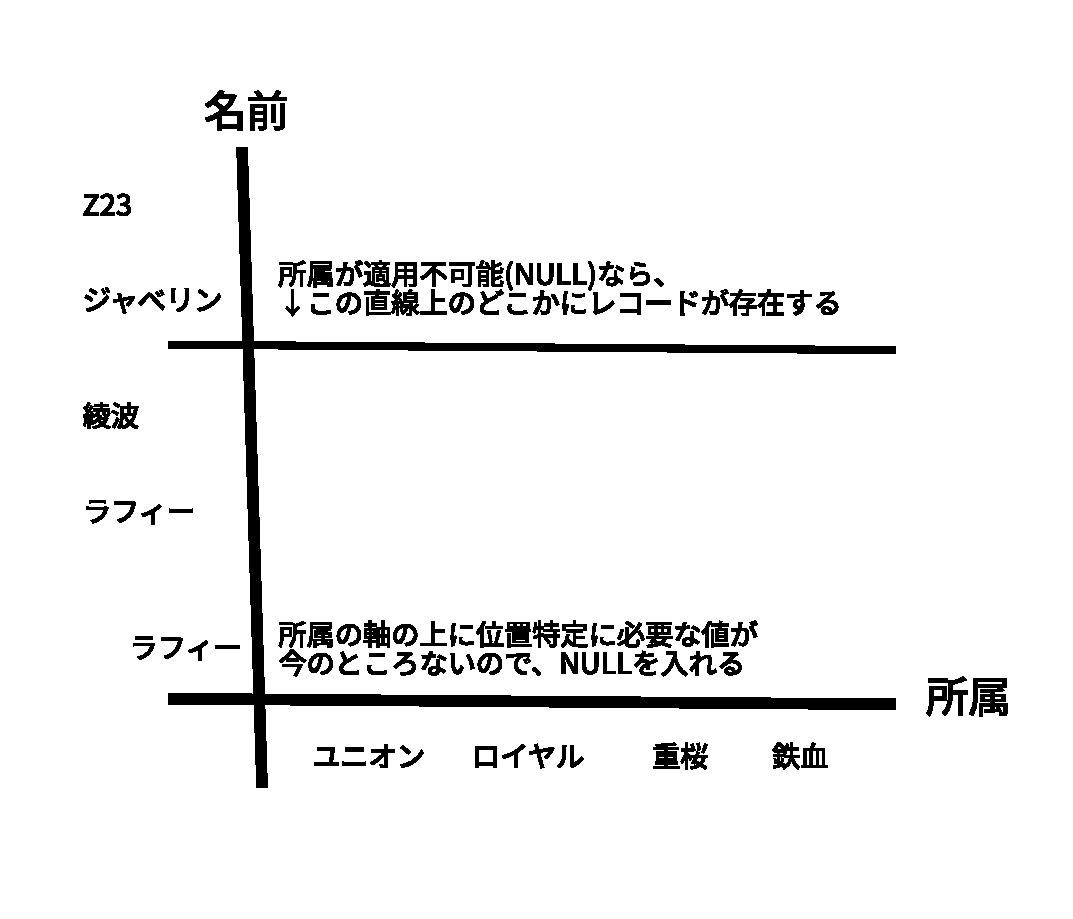
\includegraphics[width=12cm,clip]{draw/not_attach.eps}
	\caption{適用できないNULLと座標}
	\label{fig:not_attach}
\end{figure}

適用できない、というNULLの場合、レコードは、名前の座標上の特定の点を通り、所属の座標軸に平行な直線上のどこかには存在しています。ですが、場所を特定するのに必要な、所属の座標上の値が定義されていない、と解釈します。

テーブルという空間のなかで、レコードが存在している範囲は、どちらの解釈でも同じです。ですが、この範囲内のどこかに存在する、この範囲内のどこにあるか特定するのに必要な値が定義されていない、という文脈上の相違が生じます。これも、文脈的な解釈であって、SQLにはそれを区別するロジックはありません。

\subsection{NULLは使うべきか}

リレーショナルデータベースを説明する文脈でNULLが出てくるとき、多くの場合、NULLには否定的な説明がされます。また、NULLを許容したテーブルにすべきかは、しばしば宗教的な論議を呼びます。そもそもNULLは、あってはならないもなのなのでしょうか。

これは筆者の私見も入りますので、その点はご了承ください。筆者は、必要に応じてNULLは積極的に使っていくべきと考えています。その理由として、NULLとは、それに関しては知らない、という情報をあらわす値であるからです。

また、NULLは、適用できない、という情報を著わす値でもあります。特に、左右の外部結合を行う場合にはさけられないものです。そして、マスタに適用できる情報が無かった、という情報を表す値です。

これらの、知らない、適用できない、という情報を活かすのであれば、NULLは無理に忌避する必要は無いと、筆者は考えています。

その一方、NULLは、情報が無いという情報なのか、情報を入れ忘れているのか、という区別ができないという問題があります。そのため、ロバストネスなシステムを構築する、という観点からは、極力使用すべきではない、という思想もあります。
NULL以外の何らかの値が必須であるアトリビュートについては、NOT NULL属性を付けて、NULLの入力を禁じておくべきでしょう。



\section{NULLと三値論理}

NULLを、知らない、と解釈するとき、これを、真偽がわからないことをあらわす第三の値として用いることができます。つまり、TrueとFalseとUnknownで、真偽と、それが不明であることをあらわします。このとき、NULLは、真か偽か知らない状態、という値として解釈します。

真と偽、という二つの値で論理式を、二値論理と呼んでいます。それに、知らない、という第三の値をくわえたものが三値論理です。では、三値論理の真偽値はどのように考えるのでしょうか。

ここでは、Unknownの概念を論理演算に持ち込んだ、クリーネの強三値論理について説明をします。

\subsection{NULLの考え方}

三値論理では、NULLがあらわす、知らない、という情報をどのように扱うのでしょうか。
NULLは、TrueかFalseかの特定がされていない状態を表します。そして、実際にはTrueとFalseのどちらの可能性もある値として扱われます。

そのため、三値論理の論理演算の結果は、NULLが実際にはどんな値であるか特定されても結果が変化しなければ、TrueかFalseかになります。逆に、特定されることで結果が変わる場合は、結果が分からない、という意味で、NULLとなります。



\subsection{三値論理の記号}

ここでは、三値論理でとりうる値として、TrueとFalsという定数を、真偽をあわらす値として、二値論理から導入します。さらに、NULLがあらわす、知らない、という情報を表す定数として、Unknownを導入します。式では、それぞれ、TとFとUであらわします。

\subsection{NOT演算}

まず、三値論理の論理演算の基本として、否定であるNOT演算をみてみましょう。
Unknownの否定は、Unknowoになります。Knownではありません。なにより、三値論理には、Knownという値はありません。

Unknownは、TrueかFalseかを知らない、という意味です。そのため、Unknownで隠されている値がTrueかFalseか特定されない状態で否定しても、その結果がTrueなのはFalseなのかが決定できません。つまり、Unkonwnの否定を取ってもUnknownになってしまう、ということです。

\begin{table}[htb]
  \begin{tabular}{|c|c|} \hline
    $A$ & $\lnot A$ \\ \hline
    $T$ & $F$ \\
    $F$ & $T$ \\
    $U$ & $U$ \\ \hline
  \end{tabular}
  \label{chart:not}
  \caption{$\lnot A$の真理値表}
\end{table}



\subsection{OR演算}

三値論理のOR演算は、TrueとUnknownの間ではTrueになります。これは、TrueとOR演算をすれば、Unknownが実際にはTrueであってもFalseであってもTrueとなるためです。

また、FalseとUnknownの間では、Unknownになります。これは、UnknownがTrueであればTrue、FalseであればFalseで、結果が変化するためです。

UnknownとUnknownの間のOR演算は、Unknownになります。これは、実際の値がTrueかFalseかが特定できないため、OR演算の結果も特定できないためです。

\begin{table}[htb]
  \begin{tabular}{|c|c|c|} \hline
    $A$ & $B$ & $A \lor B$ \\ \hline
    $T$ & $T$ & $T$ \\
    $T$ & $F$ & $T$ \\
    $T$ & $U$ & $T$ \\
    $F$ & $T$ & $T$ \\
    $F$ & $F$ & $F$ \\
    $F$ & $U$ & $U$ \\
    $U$ & $T$ & $T$ \\
    $U$ & $F$ & $U$ \\
    $U$ & $U$ & $U$\\ \hline
  \end{tabular}
  \label{chart:or}
  \caption{$A \lor B$の真理値表}
\end{table}


\subsection{AND演算}

AND演算は、TrueとUnknownの間ではUnknownになります。これは、UnknownがTrueかFalseかで結果が変化するためです。

また、FalseとUnknownとの間のAND演算は、必ずFalseになります。これは、Unknownの値にかかわらず、FalseとのAND演算の結果は、かならずFalseとなるためです。

UnknownどうしのAND演算は、結果がUnknownとなります。これは、TrueかFalse可が特定できないので、演算の結果を特定できないためです。

\begin{table}[htb]
  \begin{tabular}{|c|c|c|} \hline
    $A$ & $B$ & $A \land B$ \\ \hline
    $T$ & $T$ & $T$ \\
    $T$ & $F$ & $F$ \\
    $T$ & $U$ & $U$ \\
    $F$ & $T$ & $F$ \\
    $F$ & $F$ & $F$ \\
    $F$ & $U$ & $F$ \\
    $U$ & $T$ & $U$ \\
    $U$ & $F$ & $F$ \\
    $U$ & $U$ & $U$\\ \hline
  \end{tabular}
  \label{chart:and}
  \caption{$A \land B$の真理値表}
\end{table}


\subsection{論理包含}

論理包含とは、$A \to B$ と記載します。
AならばBと読み下し、Aという命題と、Bという命題の関係をあらわすものです。
論理包含は、AがTrueのときのみBの真偽を判定する、という言い方もできます。AがFalseであれば、論理包含の結果はTrueとなります。

論理演算の書き方をすると、式\ref{equ:implication}のように書きなおせます。

\begin{equation}
\label{equ:implication}
A \to B = \lnot A \lor B
\end{equation}

たとえば、哺乳類は動物である、という命題をA、パンダは動物である、という命題をBとします。
このとき、哺乳類は動物であるという命題がTrueなので、パンダが動物であるかという命題の結果を、$A \to B$の値とします。
そんため、この例では、$A \to B$がTrueとなります。

もし、Aが哺乳類は植物である、という命題であれば、AはFalseなので、Bの真偽にかかわらず、$A \to B$はTrueとなります。このTrueは、命題AがFalseなので結論が出ない、という意味のTrueです。

\subsubsection{三値論理の論理包含}
三里値論理での倫理包含とは、命題のいずれかがNULLである、つまり、答えが分からない命題があるときに、ならば、という関係に真偽が付けられるのか付けられないのか、ということでもあります。

これまでの、三値論理でのNOTとORから、論理包含の真理値表を作ることができます。

\begin{table}[htb]
  \begin{tabular}{|c|c|c|} \hline
    $A$ & $B$ & $A \to B$ \\ \hline
    $T$ & $T$ & $T$ \\
    $T$ & $F$ & $F$ \\
    $T$ & $U$ & $U$ \\
    $F$ & $T$ & $T$ \\
    $F$ & $F$ & $T$ \\
    $F$ & $U$ & $T$ \\
    $U$ & $T$ & $T$ \\
    $U$ & $F$ & $U$ \\
    $U$ & $U$ & $U$\\ \hline
  \end{tabular}
  \label{chart:impliment}
  \caption{$A \to B$の真理値表}
\end{table}



ここで気をつけるのは、$U \to U$の値はUであるということです。本来、$A \to A$の値はAの値と一致します。これは同語反復と呼ばれる性質です。

Uは、わからない、という意味です。これは、真偽が分からない、という意味であると同時に、そもそもどんな命題なのかが分からない、という解釈をすることができます。そう考えたとき、$\to$の左右のUは、同じ命題なのか違う命題なのか、その判断ができないことになります。

そう考えたとき、$U \to U$の値は、TrueとFalse全ての組み合わせを考慮する必要があり、結果的にUnknownとするのが自然であると考えることができます。